%% Copernicus Publications Manuscript Preparation Template for LaTeX Submissions
%% Please use the following documentclass and journal abbreviations for preprints and final revised papers.
%% 2-column papers and preprints
\documentclass[gmd, manuscript]{copernicus}
%% \usepackage commands included in the copernicus.cls:
%\usepackage[german, english]{babel}
%\usepackage{tabularx}
%\usepackage{cancel}
%\usepackage{multirow}
%\usepackage{supertabular}
%\usepackage{algorithmic}
%\usepackage{algorithm}
%\usepackage{amsthm}
%\usepackage{float}
%\usepackage{subfig}
%\usepackage{rotating}
\usepackage{enumitem}

\usepackage[colorinlistoftodos,textwidth=0.4in,textsize=tiny]{todonotes}

\begin{document}

\title{Applications of Machine Learning and Artificial Intelligence in Tropospheric Ozone Research}

\Author[1]{Sebastian H. M.}{Hickman}
\Author[2]{Makoto}{Kelp}
\Author[3]{Paul}{Griffiths}
\Author[4]{Kelsey}{Doerksen}
\Author[5]{Kazuyuki}{Miyazaki}
\Author[5]{Elyse}{Pennington}
\Author[6]{Gerbrand}{Koren}
\Author[7]{Fernando}{Iglesias-Suarez}
\Author[8]{Martin}{Schultz}
\Author[9,10]{Kai-Lan}{Chang}
\Author[9]{Owen R.}{Cooper}
\Author[3]{Alex}{Archibald}
\Author[11,12]{Roberto}{Sommariva}
\Author[13]{David}{Carlson}
\Author[14]{Hantao}{Wang}
\Author[14]{Jason}{West}
\Author[15]{Zhenze}{Liu}


\affil[1]{Chemistry Dept, University of Cambridge}
\affil[2]{Doerr School of Sustainability, Stanford University, CA, USA}
\affil[3]{National Centre for Atmospheric Science, Cambridge University}
\affil[4]{Department of Computer Science, Oxford University}
\affil[5]{Jet Propulsion Laboratory, California Institute of Technology, Pasadena, CA, USA}
\affil[6]{Copernicus Institute of Sustainable Development, Utrecht University, Utrecht, the Netherlands}
\affil[7]{Predictia Intelligent Data Solutions S.L., Santander, Spain}
\affil[8]{J\"ulich Supercomputing Centre, Forschungszentrum J\"ulich, J\"ulich, Germany}
\affil[9]{NOAA Chemical Sciences Laboratory, Boulder, CO, USA}
\affil[10]{Cooperative Institute for Research in Environmental Sciences, University of Colorado Boulder,}
\affil[11]{ School of Geography, Earth and Environmental Sciences, University
of Birmingham, Birmingham, UK}
\affil[12]{School of Chemistry, University of Leicester, Leicester, UK}
\affil[13]{Civil and Environmental Engineering, Duke University, NC, USA}
\affil[14]{Department of Environmental Sciences and Engineering, University of North Carolina, Chapel Hill, NC, USA}
\affil[15]{Jiangsu Key Laboratory of Atmospheric Environment Monitoring and Pollution Control, School of Environmental Science and Engineering, Nanjing University of Information Science and Technology, Nanjing, China}
\affil[*]{These authors contributed equally to this work.}

%\correspondence{NAME (EMAIL)}

\runningtitle{TOAR-ML4O3}
\runningauthor{TEXT}
\firstpage{1}

\maketitle

\begin{abstract}
TEXT
\end{abstract}
\listoftodos

%\copyrightstatement{TEXT} %% This section is optional and can be used for copyright transfers.
%% LITERATURE CITATIONS
%%
%% command                        & example result
%% \citet{jones90}|               & Jones et al. (1990)
%% \citep{jones90}|               & (Jones et al., 1990)
%% \citep{jones90,jones93}|       & (Jones et al., 1990, 1993)
%% \citep[p.~32]{jones90}|        & (Jones et al., 1990, p.~32)
%% \citep[e.g.,][]{jones90}|      & (e.g., Jones et al., 1990)
%% \citep[e.g.,][p.~32]{jones90}| & (e.g., Jones et al., 1990, p.~32)
%% \citeauthor{jones90}|          & Jones et al.
%% \citeyear{jones90}|            & 1990


%%%%%%%%%%%%%%%%%%%%

\introduction  %% \introduction[modified heading if necessary]
Tropospheric ozone is a harmful atmospheric pollutant and an important greenhouse gas, contributing to both environmental and public health issues. Long-term exposure to elevated ozone levels is linked to hundreds of thousands of premature deaths globally each year \citep{malashock_global_2022, malley_updated_2017, health_effects_institute_state_2024}. Short-term exposure can cause serious negative health impacts \citep{bell_who_2014} including reduced lung function, particularly in individuals with pre-existing medical conditions \citep{us2020integrated}. Beyond its health impacts, tropospheric ozone significantly damages vegetation in natural ecosystems and agricultural fields \citep{mills_ozone_2018}. In addition, ozone plays a critical role in tropospheric chemistry, both as a source of oxidants and as a primary oxidant itself \citep{monks_tropospheric_2015}.

Ozone is not directly emitted into the troposphere but is photochemically produced in the presence of sunlight by reactions involving its precursor gasses: carbon monoxide (CO), methane (CH$_4$), volatile organic compounds (VOCs), and nitrogen oxides NO$_X$ (NO$_X$, NO+NO$_2$). In addition, ozone is transported from the stratosphere into the troposphere. The removal of tropospheric ozone is controlled by chemical loss and deposition to the surface \citep{archibald_tropospheric_2020}. The lifetime of ozone in the troposphere ranges from days to weeks, depending on local chemical and meteorological conditions \citep{lelieveld_what_2000, monks_tropospheric_2015}. This variability allows ozone and its precursors to be transported over long distances from their sources \citep{fiore_multimodel_2009}.

Modeling tropospheric ozone is a challenging task due to the complex coupling of chemical and physical processes that control its local concentrations across different spatial and temporal scales, as detailed in Figure \ref{fig:difficulties1}. Traditionally, concentrations of ozone and other chemical species are calculated using numerical models of the atmosphere that represent these processes across a wide range of spatial scales, from high-resolution urban models (meter-scale) to global chemistry-climate models with resolutions ranging from tens to hundreds of kilometers (e.g. \citet{Morgenstern2017}). 

\todo[inline]{Text for Figure zero here?}
\begin{figure}
    \centering
    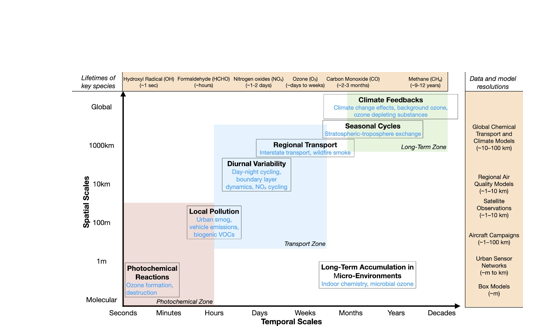
\includegraphics[width=1.05\linewidth]{figures/Figure0.png}
    \caption{Spatial and temporal scales of tropospheric ozone chemistry processes. The x-axis shows timescales, from rapid photochemical reactions to long-term climate feedbacks, and the y-axis shows spatial scales, from local pollution to global atmospheric transport. Species lifetimes and relevant data sources and models are displayed to illustrate the range and scales of phenomena and methods used to study ozone chemistry.}
    \label{fig:difficulties1}
\end{figure}
\todo[inline]{Text for Figure one here?}
\begin{figure}
    \centering
    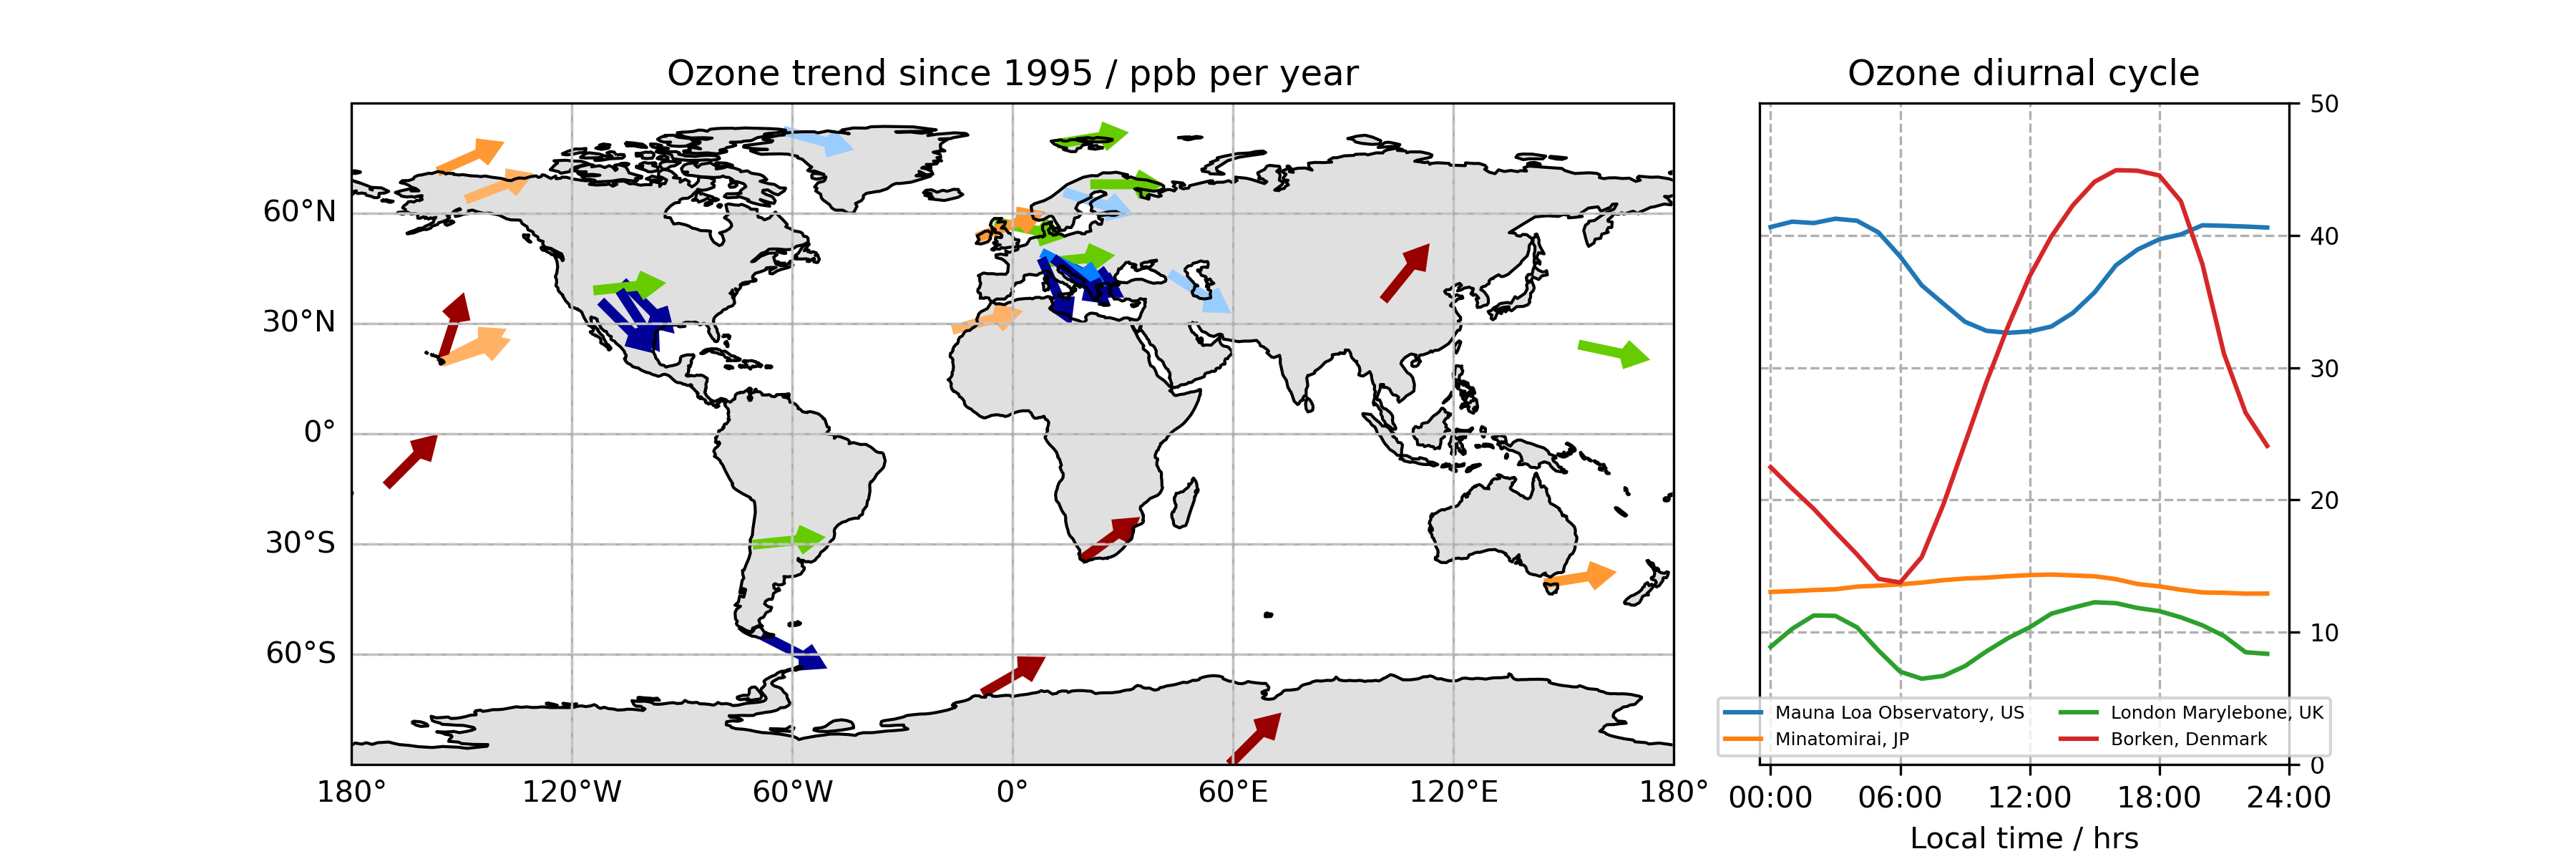
\includegraphics[width=1.05\linewidth]{figures/figure1.png}
    \caption{Diversity in ozone}
    \label{fig:difficulties2}
\end{figure}

Despite the success of ozone simulations in air quality and climate research, there are still challenges to reach accurate simulations of ozone \citep{young_tropospheric_2018}. For example, although ozone is the longest and most measured trace gas in our observational record, large uncertainties still exist in global model estimates of tropospheric ozone and its trends. Observations from ground stations, ozonesondes, and satellites indicate that tropospheric ozone has generally increased in recent decades \citep{ziemke_trends_2019, young_tropospheric_2018, IPCC_2021_WGI_Ch_2}. While global atmospheric chemistry models agree that the global tropospheric ozone burden has increased from pre-industrial times to the present day, they vary regarding the spatial distribution and magnitude of the increase \citep{skeie_historical_2020, christiansen_multidecadal_2022, fiore_understanding_2022}. Potential sources driving this model bias include uncertainties in tropical emissions \citep{zhang_contributions_2021}, nonlinear NO$_X$-VOC chemistry (Shah et al 2023), stratosphere-troposphere exchange \citep{neu_tropospheric_2014}, boundary layer mixing \citep{lu_exploring_2019}, missing chemical mechanisms such as halogen chemistry \citep{wang_active_2015}, and deposition \citep{clifton_dry_2020}. 

Machine learning (ML) approaches, which can learn and reproduce nonlinear characteristics of a system from data \citep{hornik_multilayer_1989}, may provide a valuable complement to physical models. As the quantity and quality of observational data on ozone \citep{Schultz2017} and on the broader Earth system \citep{doi:10.1080/17538947.2016.1250829,reichstein_deep_2019} continue to grow, ML is becoming an increasingly viable tool for advancing ozone research. While most ozone ML studies to date have prioritized prediction, ML also has great potential to enhance process-level understanding. Observational data, when integrated with model simulations through data assimilation techniques, have already improved our understanding of emissions and atmospheric chemistry by reducing uncertainties (Miyazaki et al., 2020). ML can complement these efforts by combining observational data with model outputs, emulating model components, or enabling computationally cheaper simulations, thereby efficiently diagnosing sources of error in global atmospheric models and improving tropospheric ozone estimates. In addition, ML presents advantages over traditional numerical models, particularly in terms of computational efficiency and in the ability to learn from large datasets, as demonstrated by the success of data-driven nowcasting and weather forecasting models \citep{bi_accurate_2023, lam_learning_2023, price_gencast_2024}. However, ML also has limitations, such as challenges in generalization, validation, and interpretability. Addressing these issues may be particularly relevant for the ozone modeling community where both predictive accuracy and physical understanding are valued.
 
In this Perspective, we provide an overview of the state of ML in tropospheric ozone research, review previous applications of ML to various problems related to ozone, and discuss persistent challenges and emerging opportunities. We detail the bottlenecks to progress in applying ML to ozone problems, including the limitations of available training data, heterogeneity of data sources, and computational limits. We suggest that the use of ML can provide tangible improvement over existing methods in some aspects of ozone research and we provide possible paths towards further improvement to complement existing models and initiatives.

To date, ML for ozone has been most widely applied in three main areas: forecasts based on ground-based observations are reviewed in Section 2, methods for complementing or replacing parameterizations in numerical models of atmospheric chemistry and transport are discussed in Section 3, and ML models that are using satellite data or combined data products are presented in section 4. Limitations specific to each section are briefly mentioned, and we find common limitations across domains. Section 5 highlights and further details these cross-cutting issues and limitations with the application of ML to ozone studies, while Section 6 describes future directions for the field, highlighting emerging approaches that seek to address the cross-cutting challenges.

\todo[inline]{Text for figure 2}

\begin{figure}
    \centering
    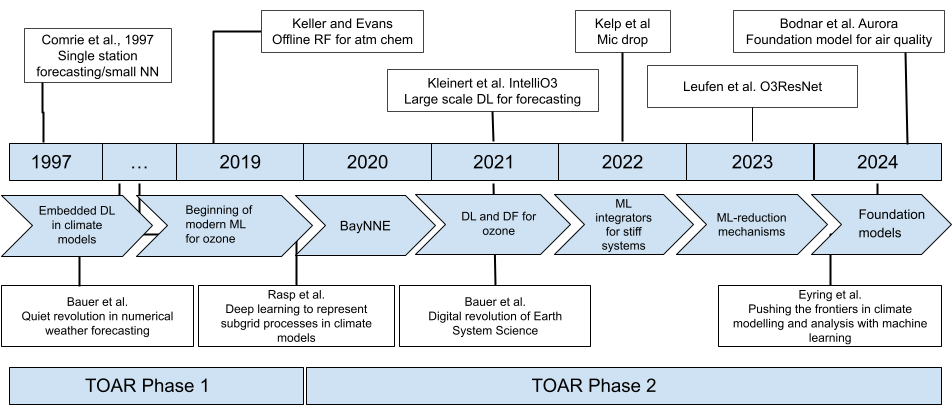
\includegraphics[width=0.95\linewidth]{figures/In progress ML4O3.png} 
    \caption{Timeline of ML / AI research as it pertains to this field etc}
    \label{fig:timeline}
\end{figure}

%%%%%%%%%%%%%%%%%%%%

\section{Applications of ML to in-situ ozone observations: short-term ground level ozone forecasting}
\label{sec:tsforecast}

\subsection{Background}
State-of-the-art air quality forecasts, typically on the timescales of hours or days and up to a few days ahead, are based on the output of numerical chemical transport models \citep{Marecal2015}. These models may be run at higher-than-usual spatial resolution for the area of interest \citep{Savage2013}, and may be post-processed to more accurately represent observations \citep{Casciaro2022}. As with other air pollutants, notably PM$_{2.5}$ \citep{Feng2015}, ML is increasingly being directly applied to the task of short-term, ground-level ozone forecasting, and to bias-correct existing air quality forecasting systems with considerable success. The availability of large and growing observational datasets has facilitated these advances \citep{Schultz2017}. Forecasting ozone concentrations as time series with ML comes with significant challenges: forecasting ozone is a spatiotemporal problem, and ozone is controlled by processes of varying spatial and temporal scales.  

Short-term forecasting of air pollutants including ozone, i.e. predictions of expected concentrations over 1-4 days, is relevant for public health and scientific questions. One important task is to provide the public with accurate and timely warnings of poor air quality, which may influence public behaviour and encourage precautions, leading to reduced exposure to poor air quality \citep{Buonocore2021, Hahm2021,Alari2021, Saberian2017}. Short-term ozone forecasting is also related to filling in missing ozone data, for example, if data is missing from an observational time series, which is an important task for analyses that require complete data. While many studies have focused on ozone forecasting, similar ML architectures and workflows have been used to fill in missing data in observational datasets \citep{betancourt_global_2022, Wu2024}. The focus on short-term present day forecasts, rather than on climate applications, means that ML methods are well suited to this task, as there are often training data available that are similar to test data. 

Many short-term forecasting studies using ML have focused on forecasting only at selected observational stations, using observed ozone and additional chemical species, and meteorological variables when they are available from individual stations or external datasets \cite{Comrie1997, cobourn_comparison_2000, Kolehmainen2001,Eslami2020, sayeed_novel_2021, leufen_o3resnet_2023, Hickman2023}, which provide measured time series of ozone and perhaps other chemical species or meteorological variables. This approach has the advantage of forecasting high-fidelity data, allowing modelers to improve the forecasting model through systematic comparison against observations or through data assimilation. Furthermore, since it is difficult to downscale a relatively coarse chemical transport model (CTM) at specific locations, using time series data from a particular station is an attractive way to make predictions at particular locations. However, approaches of this kind do not necessarily provide ozone forecasts across all locations that we may be interested in, as a gridded model product model might.

\subsection{Progress and State of the Science}

As with other fields, the advances in ML-based ozone forecasting have been pushed by developments on two axes - first, increasing quantities of data and second, larger models with more appropriate inductive biases. The field has a long history (see Figure \ref{fig:timeline}), with studies being published even during the most recent artificial intelligence (AI) "winter", beginning with a feed-forward neural network (NN) in 1996 \citep{Yi1996}. \citet{Comrie1997} illustrated that a neural network (NN) could be used to forecast ozone at eight stations in the USA. This was followed by further feed-forward NN approaches, often with datasets drawn from a single location or city \citep{cobourn_comparison_2000, Kolehmainen2001}. Neural methods were typically evaluated in comparison with (autoregressive) regression models, often finding that NNs were better able to forecast ozone concentrations and extrema on the test data \cite{Nunnari1998, Schlink2003, Chaloulakou2003}, although the improvement was often only marginal. Alongside the successes of feed-forward NN architectures, other work drew attention to methods seen to be more interpretable, such as fuzzy logic systems and regression trees \citep{Gardner2000, heo_new_2004}. Other work leveraged methodological advances in ML architectures designed for temporal data, including the use of recurrent neural networks (RNNs) and convolutional neural networks (CNNs) to account for lagged relationships in the time series data \citep{Eslami2020, sayeed_novel_2021, Kleinert2021}. Recent work has combined architectures to model the relationships that control ozone, including combining components such as transformers and CNNs to account for the temporal and spatial information relevant to forecasting \citep{Chen2022, cheng_spatio-temporal_2022, han_capability_2023}. However, datasets have typically been limited to single countries or cities, due to the lack of a combined database of station measurements. The introduction of the Tropospheric Ozone Assessment Report (TOAR) surface database \citep{Schultz2017} and the TOAR-II database have facilitated recent studies on data drawn from multiple countries \citep{leufen_o3resnet_2023, Hickman2023}. The importance of curation of large datasets for scientific progress in ML is highlighted below in the Outlook section. 

Increasingly, more complex architectures are being used to enhance the accuracy of ozone forecasts, and more data are being included as input to the models. The inputs that are relevant to the physical drivers of ozone concentrations, such as past observations of ozone and covariates, and nearby covariates, reflect processes that control ozone observations, and feasibly contribute to improved ozone forecasting and infilling. Recently we have seen methods on the scale of the ML architectures and data used for weather forecasting \citep{bi_accurate_2023, lam_learning_2023}, transferring to ozone forecasting by leveraging very large datasets and models, as ozone concentrations are controlled in part by meteorological factors. In weather forecasting there is work on forecasting at observation stations using these methods, and transferring these methods to forecast ozone at ground-level stations is feasible \citep{manshausen_generative_2024}. 

General trends have emerged from recent forecasting studies with ML. Typically, models trained on many sites perform better than models trained to predict ozone at a single station, and larger deeper models are better able to forecast given sufficient data. However, it is difficult to determine precisely which individual features of models are contributing most to improved accuracy as studies typically use different test data. The establishment of a robust benchmark dataset, which could be used across the community to evaluate the performance of different methodologies would allow rigorous comparison between competing methods. A dataset of this kind for weather forecasting, WeatherBench, and its successor \citep{Rasp2020, Rasp2024} continue to facilitate effective inter-comparison between different ML and numerical models. A similar dataset to perform the same function for ozone forecasting would allow the robust comparison of different methods, and may guide the field towards more accurate models. This benchmark dataset would need to cover a range of environments, including extreme events. Careful curation and data fusion of the TOAR surface ozone database with other relevant datasets might provide a robust and representative benchmark dataset, building on existing work \citep{Betancourt2021}.

\subsection{Future Outlook}
While forecasting ground-level ozone has seen some successes, there are still some necessary steps before we have reliable operational ML forecasts. As in other fields, the community has seen improved performance with scaling datasets, and training across a variety of environments with rich data \citep{leufen_o3resnet_2023}. While  the TOAR database of surface observations provides a large collection of in-situ data, the community is still missing a benchmark dataset that could be used to robustly compare methods \citep{Dueben2022, Rasp2024}, and explore model deficiencies. Creating this dataset should be a collaborative effort that may provide the step-change in ground level air pollution forecasting that other benchmark datasets have precipitated in other fields \citep{Deng2009}. Part of this benchmark should focus on extreme events and probabilistic metrics, as currently the community does not evaluate performance on extremes thoroughly, and encouraging probabilistic models and metrics may improve performance on extremes. While generalization is less of an issue for short-term forecasting, building models that can generalize to undersampled regions of the world would facilitate better pollution forecasting in countries with fewer data. Finally, work on interpretability and explainability is limited, and further study may give more insight into the internal working of these models, and possibly insight into physical processes.


\section{Applications of ML methods in atmospheric chemical modeling}
\subsection{Background}
Global modeling of atmospheric chemistry is a grand computational challenge due to the high dimensionality of coupled chemical species, the nonlinearity and numerical stiffness of solving chemical mechanisms, and interactions with transport on all scales. The inclusion of comprehensive atmospheric chemistry in Earth system models (ESMs)—which simulate the interactions between the atmosphere, oceans, land surface, and biosphere—is a priority science frontier \citep{national_research_council_national_2012}. Atmospheric chemistry in these models is typically represented by chemical transport models (CTMs), which focus on the distribution and chemical evolution of species in the atmosphere. For some applications, chemistry-climate models (CCMs) may further couple chemical processes with climate dynamics, allowing feedback between chemistry and climate. Current atmospheric chemistry models integrate the coupled chemical kinetic equations for mechanism species over model time steps using high-order implicit numerical solvers, but these solvers are computationally expensive \citep{sandu_benchmarking_1997} and often dominate the cost of an atmospheric simulation \citep{eastham_geos-chem_2018}. Such costs put the inclusion of atmospheric chemistry in tension with other computationally intensive ESM/CCM priorities such as increased spatial resolution or ensemble simulations. The current slowdown in the rate of increase in the speed of computer CPUs—the “end of Moore's law”—underscores the need for computationally efficient approaches \citep{theis_end_2017}.
 
Chemical solvers in atmospheric models compute the local evolution of species concentrations over a chemical time step that may range from minutes to hours depending on the model \citet{brasseur_modeling_2017}. The chemical mechanisms used in global/regional atmospheric models and ESMs typically include $\mathcal{O}(100)$ coupled species and is a multiscale system with chemical lifetimes ranging from less than a second to much larger than the model time step. High-order implicit solvers can integrate this system of stiff coupled differential equations with high accuracy, and fast implementations of these schemes are available, but they are still extremely costly for atmospheric models. Atmospheric models may combat that cost by decreasing the size of the chemical mechanism, breaking down the stiffness of the problem, or using lower-order approximations. However, these methods rarely achieve a speedup of more than a factor of two \citep{lin_adaptive_2023, shen_adaptive_2020} and sometimes lead to loss of accuracy in the model results. As a consequence, these computational barriers limit the ability for high-resolution simulations, detailed uncertainty analyses, and complicate the coupling of atmospheric chemistry into CCMs/ESMs for long-term climate simulations without significant compute resources. 
 
ML methods could be transformative in this area for both reducing the cost of an atmospheric chemistry simulation and facilitating their incorporation into ESMs. ML methods would seem well-suited to replace chemical solvers in atmospheric models because the chemical computation is very repetitive, involving the integration of similar conditions in neighboring grid cells and successive time steps. However, the large number of coupled species brings a ‘curse of dimensionality’ to the problem, and ML methods have no check on error growth, unlike in standard chemical solvers where errors are dampened by the negative response to perturbations (Le Chatelier’s principle). Additionally, while ML models are commonly trained and deployed using software libraries written in Python, the successful integration of ML-based algorithms and parameterizations within 3-D CTMs remains limited. A potential barrier is the difficulty of calling Python libraries from Fortran-based models, which Fortran cannot do so natively. However, recent advances in ML software can package ML code into static or dynamic libraries for flexible deployment.
                                                                             
There are a variety of examples using output from CTM and air quality models in tandem with satellite measurements, ground-level monitoring observations, meteorological reanalysis data, and emissions databases to predict or improve forecasts of ozone. These improvements can be achieved through various methods, including data fusion techniques and the creation of reduced-order models. However, because such studies involve additional data besides model outputs, they will be discussed in other sections (Section 2 and 4). Here, we emphasize studies primarily employing data from atmospheric chemical models.

\subsection{Progress and State of the Science}
Largely, ML methods in atmospheric chemistry modeling currently involve emulating model components to improve model parameterizations, reduce computational bottlenecks, and create simplified, reduced-order models. Here, emulation refers to an ML model reproducing the same calculations as a component of a complex physical or simulated system for a set of inputs. There exists a growing number of studies forecasting ozone on short- (hourly) (Yafouz et al., 2022) and longer-term (Du et al., 2022, Chen et al., 2023) timescales, spanning from city- (Ojha et al., 2021) to regional-level (Ortiz et al., 2021) spatial scales. However, few of these studies have been implemented in operational settings (i.e., within CTM, CCMs) or offer insight beyond that of traditional model-to-observation comparison methods.   

\subsubsection{ML emulation and reduced order modeling}
\citet{Xing2020} used a hierarchy of ML models containing a CNN and long short-term memory (LSTM) network to predict ozone concentrations from CMAQ model output over 7-day forecast periods.\citet{kuo_ozone_2023} investigated how accurately ML models can learn the ozone-NO$_X$-VOC chemical relationships in a chemical mechanism and found that their ML model produced distorted NO$_X$ and VOC-limited isopleths when only trained on CMAQ model outputs. \citet{kelp_online-learned_nodate} trained an NN integrator in a photochemical box model, including an encoder/decoder to decrease dimensionality, and a recursive feedback loop over 24-hr integration time to control error growth. They found that they could compress the 101-species dimension of their mechanism into 16 features without significant error penalty and avoid error growth within a selected time horizon, though error increases beyond this window. \citet{yang_atmospheric_2024} created a machine-learned surrogate for a low-dimensional (11 species) chemical box model that both compresses the dimensionality of the chemical mechanism and reduces the numerical stiffness of the problem. They achieve numerical stability within a 9-day training window but acknowledge that such an approach may be difficult for more complex and higher-dimensional chemical mechanisms. \citet{liu_2024} employed a Fourier Neural Operator with time-embedded attention to calculate chemical concentration changes as a learnable time-dependent process. They achieved higher accuracy metrics compared to standard neural operators and U-Nets in simple box model-like simulations. 

\subsubsection{ML models implemented within global CTMs}
While there is a growing literature on using ML to emulate and improve the representation of atmospheric processes, few have implemented these ML models online within CTMs/ESMs to evaluate their effectiveness. \citet{keller_application_2019} created a random forest integrator for the GEOS-Chem global 3-D CTM driven by re-analyzed meteorological data. They achieved successful short-term simulations but found large error growth after a few weeks. \citet{liu_correcting_2022} developed a gas-phase NN solver for the CMAQ regional CTM over China, combining a standard implicit solver for radicals and oxidants with an ML solver for VOCs. They achieved an order of magnitude speedup over a 1-month simulation but with error growth over remote ocean grid cells. \citet{shen_machine-learning-guided_2022} used an unsupervised ML algorithm (simulated annealing) to create submechanisms of the full chemical mechanism in GEOS-Chem for which they solve the coupled kinetic system only for the fast species in the submechanism. The computational cost of the chemical integration decreased by half and the relative difference in ozone was <0.5\% in the troposphere and <0.1\% in the stratosphere over 8-year simulations. \citet{kelp_online-learned_nodate} implemented the low-dimensional “Super-Fast” chemical mechanism in GEOS-Chem using online training of the ML emulator, achieving stable 1-year simulations for ozone prediction with less than 10\% bias compared to the reference and reducing computational cost by a factor of five. However, their ML solver had relatively lower accuracy in pristine marine regimes with lower chemical concentrations. \citet{xia_advancing_2024} implemented a self-attention transformer chemical solver online into the WRF-Chem CTM achieving an eight-time speedup over the conventional solver with an average NMB of 2.63\% for 74 species. Their approach shows promise for accurate predictions of chemical concentrations with low overhead when coupling the ML solver to the CTM, but simulations were only run for 15 days and stability over longer time scales (>1 year) remains to be seen. 

Few studies have implemented ML models directly within CTMs/ESMs to evaluate their effectiveness, although the necessary tools exist. While ML models are typically trained and deployed using Python libraries, integration of these models into CTMs remains limited because CTMs are written in Fortran, which cannot natively call Python. Current solutions include rewriting models in neural Fortran \citep{keller_application_2019}, using the C Foreign Function Interface (CFFI) to create C-style bindings for Python scripts \citep{kelp_online-learned_2022, zhong_wrfml_2023}, or packaging ML models as callable static or dynamic libraries using TorchScript and LibTorch \citep{xia_advancing_2024}. Depending on the architecture and complexity of the coupled ML model, all coupling methods result in a speedup over the conventional reference solver. (See review by \citet{de_burgh-day_machine_2023} for greater discussion on using ML for facilitating speedups and computational cost reductions in atmospheric science models). 

\subsubsection{ML modeling processes affecting ozone chemistry}
A number of ML and data-driven advances have been made for CTM modeling that are separate from creating an ML chemical solver. \citet{wiser_amore-isoprene_2023} and \citet{wang_implementation_2023} created automated chemical mechanism reduction approaches to reduce the high dimensionality of the VOC precursors of ozone and secondary organic aerosol. \citet{sturm_conservation_2022, sturm_mass-_2020} developed methods to enforce mass and stoichiometric conservation rules in outputs from ML emulators. \citet{zhu_combining_2022} trained an ML model on CTM output parameters and satellite observations from OMI to predict urban OH concentrations. \citet{huang_neural_2022} created an NN-assisted Euler integrator to speed up the iterative computations within an implicit solver routine. 

\citet{silva_deep_2019} developed an ML parameterization for ozone dry deposition velocities using surface observations that outperformed those within CTMs for certain locations. Similarly, \citet{ivatt_improving_2020} created an XGBoost model trained on ozone surface observations and data from ozonesonde networks to predict and correct GEOS-Chem model biases. \citet{liu_correcting_2022} developed a NN model to correct surface ozone in the UKESM model, finding that temperature drives biases over Northern Hemisphere continental areas while photolysis rates contribute to global ozone biases. To be sure, there is a growing literature on ML approaches for bias corrections on existing air quality modeling systems \citep{Neal2014, Borrego2011, Silibello2015}. These approaches generally learn the error between the output of a numerical model and some observations and then apply this error correction to the output of the numerical model. \citet{nowack_using_2018} used a hierarchy of ML methods to build temperature-based ozone parameterizations for climate model sensitivity simulations. \citet{colombi_why_2023} used random forests to remove the effect of weather coupled to ozone trends. \citet{Gouldsbrough2024} used a gradient-boosted tree to downscale ozone model output from the EMEP4UK CTM. \citet{ye_diagnosing_2022} used a random forest model to identify underlying causes of CTM bias in simulating daily surface ozone variability, finding that CTM underestimates in the dry deposition velocity and cloud optical depth on wet/cloudy days were the primary drivers over China. 
 
\citet{park_learned_2023} created a prototype ML discretization for a one-dimensional horizontal passive scalar advection, an operator component common to all CTMs, and achieved stability and orders of magnitude computational gain relative to the reference when coarse-grained. \citet{sturm_advecting_2023} developed a data-driven compression method for chemical tracers within a CTM and advected the compressed representation, achieving a computational gain of 1.5$\times$ without loss of accuracy. There have been developments of ML emulators in box models for organic aerosol mechanisms detailing the ML models’ accuracy with respect to interactions with ozone \citep{mouchel-vallon_toward_2023, schreck_neural_2022}.
 
The photolysis frequencies used to inform ozone concentrations, calculated from the radiative transfer components of atmospheric models, can themselves be emulated using NNs \citep{lagerquist_using_2021} and have the longest relative history of ML emulation for atmospheric modeling \citep{krasnopolsky_new_2005,krasnopolsky_decadal_2008}. Similarly, \citet{anderson_machine_2022} used a gradient-boosted regression trees methodology to develop a parametrization for the OH radical, a key driver of O3 formation, for CCM models. 


\subsection{Future Outlook and Priorities}

The near-term future of integrating ML with 3D atmospheric chemistry modeling, particularly for tropospheric ozone prediction, relies on understanding the uncertainties and limitations of ML. Such knowledge is essential for improving or approximating specific chemical parameterizations rather than attempting to replace full-scale, multiscale chemistry simulations. Priorities should include scaling regional ML models to a global context and identifying the strengths of ML (e.g., speed of operation, pattern recognition of high volumes of data) alongside its weaknesses (e.g., inability to approximate multiscale dynamics, instability over time, resource-intensive training and black box nature). 

In the context of using ML for model component emulation and replacing traditional model components, a significant roadblock has been coupled instabilities where the ML predictions accumulate errors and drift away from the reference model over time. This coupled, unstable behavior is also common with ML model emulation in weather and climate. As a result, ML approaches are increasingly used to develop end-to-end models, which take raw input data (e.g., emissions, meteorological fields) and directly predict outputs such as ozone concentrations. Although end-to-end ML models circumvent emulating specific model components and are less susceptible to short-term instabilities and operator splitting issues, these approaches also reduce the ability to track uncertainty metrics tied to physical parameters and processes.
 
Another emerging area is the use of Physics-Informed Neural Networks (PINNs), which embed physical laws into an ML model’s architecture. While ML has been used to emulate traditional numerical solvers, this approach has often sacrificed accuracy and stability over long-term timescales in exchange for faster computations. Traditional solvers, though computationally expensive, do not exhibit these error instabilities (see Le Chatelier’s principle). PINNs may offer a solution to balance speed with accuracy and have shown success in smaller-scale systems, such as single ODEs or PDEs \citep{karniadakis_physics-informed_2021}. Although their application to large groups of ODEs or in atmospheric chemistry has not yet been widely explored, PINNs may hold the potential for achieving greater accuracy than traditional solvers, possibly overcoming some of the limitations of ML approaches in atmospheric chemistry modeling. However, PINNs may not enforce physical laws perfectly and the inherent black-box nature of certain ML components limits their transparency compared to physical models, which provide clearer constraints. Therefore, while PINNs may address some computational challenges, their contribution to advancing process-level understanding in atmospheric chemistry remains uncertain.

At present, most ML models attempting to replace components of CTM/CCM parameterizations have used supervised learning methods. These methods are typically trained using chemical data from box models or other solvers, aiming to faithfully reproduce outputs given initial conditions. However, unsupervised learning, which identifies patterns or clusters in data without explicit labels, remains underexplored in this field. An emphasis needs to be placed on understanding the factors influencing ML model performance, whether it lies in the ML model architecture, the curation of the training data, or the underlying uncertainty in our physical insights of emissions, transport, and/or chemistry. To be sure, the advent of transformers and Large Language Models (LLMs) offers a new frontier for ingesting and potentially improving AI modeling of atmospheric chemistry, but it will be crucial to understand the above points before pursuing even more complicated ML model architectures.

%%%%%%%%%%%%%%%%%%%%

\section{Applications of AI/ML methods to Remote Sensing Datasets}


\subsection{Background}
The large quantity of satellite and remote sensing data produced on a now-daily basis from polar and geostationary-orbiting satellites enables an improved understanding of the spatiotemporal distributions of ozone and the processes controlling it. Satellite remote sensing is preferred to in-situ measurements for observing ozone in the free troposphere, since it has advantages of continuous monitoring and extensive spatial coverage (Xu et al, 2024). Particularly over remote areas, satellite remote sensing may provide some insight into the distribution of ozone, and may be used to estimate ozone concentrations in locations where ground-based ozone monitoring is sparse. This is especially valuable, as CTMs depend on the representation of chemical and physical processes, and on emission inventory data, which can be difficult to obtain, and often have low temporal resolution (Yan et al, 2024). Over the past several decades, a large number of satellite instruments have been used to monitor the spatiotemporal distribution of ozone precursors and ozone in the free troposphere both regionally and globally (Fishman et al., 1990; Kim et al., 2006; Liu et al., 2010; Souri et al., 2017; Ziemke et al., 2019 ). Satellites can have both passive and active remote sensing capabilities, where passive sensors typically measure ozone through UV and thermal infrared (TIR) radiation, while ozone precursors, NO$_X$ and VOCs, are measured with spectrometers giving ultraviolet/visible nadir measurements. 

Payloads onboard polar-orbiting spacecraft used for ozone monitoring include the non-exhaustive list of: solar backscatter ultraviolet and total ozone mapping spectrometer (TOMS) (Heath et al. 1975), stratospheric aerosol and gas experiment (SAGE) (McCormick et al 1979), scanning imaging absorption spectrometer for atmospheric cartography (SCIAMACHY) (Bovensmann et al. 1999), Ozone Monitoring Instrument (OMI) (Levelt et al 2018), Total Ozone Unit (TOU) (Wang et al 2010) and Solar Backscatter Ultraviolet Sounder (SBUS) (Huang et al 2012) aboard the FengYun satellites, Environment Monitoring Instrument (EMI) and its follow on EMI-2 (Zhao et al 2020, Chen et al 2022), Global Ozone Monitoring Experiment (GOME) and its follow-on GOME-2 (Burrows et al 1999, Munro et al 2016) and the latest Sentinel-5P Tropospheric Monitoring Instrument (TROPOMI) (Veefkind et al 2012).

Geostationary payloads include the Tropospheric emissions: monitoring of pollution (TEMPO) (Naeger et al., 2021), geostationary environment spectrometer (GEMS), and the Sentinel-4 instrument on Meteosat Third Generation Sounder (MTG-S). Recent advancements in satellite measurements, including sensors with enhanced accuracy, such as TROPOMI, and high resolution geostationary satellites such as GEMS and TEMPO are currently providing unprecedented information on atmospheric composition (Yang et al, 2021). In the context of estimating surface ozone concentrations, these satellites contribute by measuring ozone precursors with improving accuracy. Furthermore, IASI and GOME-2, and TES/OM provide lower tropospheric ozone retrievals. 

ML and deep learning offer several advantages over CTMs for estimating ozone concentrations based on indirect measurements from satellites, including enhanced computation efficiency and the ability to capture non-linearity and reveal hidden patterns in large datasets (Ghahremanloo et al., 2021a). ML combined with remote sensing data has been used for ozone profiles and ML-informed estimation of surface ozone, which we introduce in the following section.
\subsection{Progress and State of the Science}
\subsubsection{Machine learning for ozone retrieval}
Ozone retrieval is the task of estimating ozone profiles from spectrometers on satellites, which measure radiance spectra from the atmosphere. Usually carried out with numerical calculations based on physics, using ML for ozone retrieval is a burgeoning field. The task is to take level 1 radiance data from the satellites and to produce a level 2 product detailing an ozone profile.

The dominant ML architecture in ozone retrieval studies with remote sensing data has been decision tree-based methods, chosen for their relative simplicity to implement and feature interpretability. TROPOMI in combination with OMI were used with a Random Forest model to estimate ground-level ozone concentrations in California at a 10km resolution by Wang et al (2022). Zhu et al (2022) applied random forests to the OMI OMPROFOZ product in combination with meteorological conditions, land-use information and proxies of anthropogenic emissions as their predictors for estimating long-term spatiotemporal patterns of surface ozone concentrations in China over 2005-2019. Extreme Gradient Boosting (XGBoost) was used by Liu et al (2020) to predict MDA8 with ozone retrievals, aerosol reanalysis, meteorological parameters and land-use data on a national scale, highlighting their model’s robustness and reliability for historical data prediction from 2013-2017. Yao et al (2024) leveraged Light Gradient Boosting (LightGBM) with SHAP values with the TROPOMI satellite observations for ozone retrieval in Hangzhou Bay, China.  
\subsubsection{Machine learning for surface ozone estimation using satellite data}
More recently, Deep Learning has been leveraged for ozone estimates for its ability to handle complex and unstructured data, without the need for additional processing into tabular or other structured formats commonly needed for ML models. Müller et al (2002), developed a feed-forward neural network scheme for retrieving total ozone columns from the Global Ozone Monitoring Experiment, showing general agreement with TOMS and GOME level-3 maps. Ghahremanloo M. et al. (2023) used a Deep-Convolutional Neural Network (CNN) with TROPOMI to estimate MDA8 in the contiguous United States at a 4km-spatial resolution in 2019, and included the SHAP explanations to provide feature explainability. Zhu et al (2022) used a Deep Forest (Zhou et al, 2017) architecture to estimate surface O3 from the TROPOMI level-3 O3 columns in Chongqing.  Zong et al (2024) also used a Deep Forest in their study with satellite ozone concentrations from TROPOMI, comparing their method to six other models: RF, CatBoost, XGBoost, LightGBM, Decision Tree and Gradient Boosted Decision Tree. The authors found that the Deep Forest showed significant advantages over other shallower, tree-based regression models. Zang et al. (2021) employed a deep learning approach with a tree-based ensemble architecture named semi-SILDM for predicting ozone at national (5km) and urban (250m) scaled in China with the Moderate Resolution Imaging Spectroradiometer (MODIS) Top of Atmosphere (TOA) measurements. To address sparse in situ measurement data, Luo et al. (2022) developed a two-stage deep learning model called ExDLM with MODIS MOD02SSH products, O3 precursors, ancillary data and meteorological variables to interpret the dynamics of O3 during extreme weather and clean days in Beijing, providing greater spatial and temporal accuracy than current models. 
\subsubsection{Combining Data Assimilation, CTMs and Satellite Observations}
The combination of satellite products, CTM and data assimilation outputs as inputs into ML models has also been explored for ozone estimation. Qian, et al. (2016) proposed a hybrid neural network model using satellite-based data from OMI and OMDOAO3e, GEOS-Chem CTM outputs, ozone vertical profiles, meteorological variables, land-use terms and other atmospheric compounds for predicting 8hr max ozone in the continental United States between 2000-2012. Yan et al. (2024) combined data assimilation data from ERA5 with observations from the Himawari-8 satellite, in addition to proposing a joint linear regression and deep learning model to capture the linear and nonlinear relationships between inputs and near-surface ozone concentration simultaneously in China. Their work showcases the potential for utilizing combined data sources and combined methodologies for their respective strengths in modeling ozone, and addresses the need for high temporal resolution ozone monitoring that remote sensing can provide.
\subsubsection{ML for Remote Sensing Processing}
ML can also be used as a data processing tool to compensate for combat missing and low resolution data from remote sensing products caused by cloud cover and high signal-to-noise-ratio of older instruments. Imputation for OMI-NO2 columns has been achieved through the use of a full residual network in (Li and Wu, 2021) and similar methodology by Xi et al., (2023), who then further developed a 3D Convolutional Neural Network using the processed NO2 for daily maximum 8h average ozone concentration over China from 2016 to 2020. 3-D CNN’s have the ability to compute features from the spatial and temporal dimension by convolving a 3-D core (Ji et al 2013), which can extract spatiotemporal information and improve ML model robustness. Jung et al (2024) used the XGBoost algorithm with OMI and MODIS products with meteorological variables and land-use data to estimate MDA8 at a 1km resolution during 2004-2020 in Taiwan, and used a Random Forest model to impute the missing values of the satellite-based measurements. Shi et al (2024) developed an ozone column harmonization method using a ConvNeXt (Liu et al 2022) neural network architect to reconstruct high-resolution ozone column concentration products for the Tibetan Plateau from 2004-2022. The authors used the neural network to learn the mapping relationship between OMI (which offers a long data record but with high signal-to-noise ratio) and Sentinel-5P TROPOMI (which offers a high spatial resolution but relatively short data record), creating a reconstructed ozone column concentration product with the long length of OMI availability and high spatial resolution and accuracy characteristics of TROPOMI. 

\subsection{Future Outlook and Priorities}
As with the integration of ML with atmospheric chemistry 3-D modeling, priorities in the domain of ML with remote sensing should focus on the movement from regional to global, geographically-generalizable models. Remote sensing datasets are largely available on a global scale, but ML models in this context are limited due to lack of adequate ground truth. The inclusion of tropospheric ozone domain experts is critical to the correct evaluation of models where ground truth is not available to assess performance as compared to CTMs. 

Data harmonization and data fusion with ML will be valuable to the remote sensing community to extend the dataset availability as old instruments are retired and new instruments are launched. Particularly for Deep Learning, of which model performance is often dependent on training dataset size, it will be vital to develop methods to harmonize data from older ozone monitoring instruments with the latest payloads to extend study periods for long-term trend analysis. 

Remote sensing with ML offers the ability to investigate the linear and non-linear processes of ozone at higher spatiotemporal resolutions than ground-based measurements and CTM estimates, but the value of both methodologies should not be understated. Instead of using one method over another, research into hybrid physical-ML modeling for ozone retrieval can improve prediction performance, inference efficiency and interpretability (Willard et al, 2022). The merging of principles from AI and simulation domains has the potential to improve scientific understanding of ozone formulation by leveraging the strengths of both methodologies to utilize the latest high-resolution remote sensing data with large volumes of pre-existing historical datasets.

%%%%%%%%%%%%%%%%%%%%

\section{Challenges and Limitations}
In this section we reflect on some common challenges and limitations for using AI in the context of ozone forecasting, modeling and observations. 
\subsection{The challenges of data: data quality, benchmarks and harmonized datasets}
In the field of air pollution and atmospheric composition research, the use of ML is hampered by the absence of benchmark datasets suitable for training different model types with varying size and complexity. Such well-defined benchmarks including datasets, training objectives, evaluation scores, and baseline models have been instrumental for the rapid development of ML models in other fields  [Dueben et al., 2022]. Benchmark datasets,  specifically,  WeatherBench (Rasp et al., 2020) and Weatherbench2 (Rasp et al., 2024), have been a key factor driving the transformation of ML  weather forecasting between 2022 and 2024. 

Whilst the breadth of information available in datasets like TOAR, GHOST and reanalysis products like CAMS and TC are vast, these products provide significant challenges to the development of ML models for ozone due to heterogeneous data formats and lack of succinct documentation that focuses on the use of such data for ML applications. Hence, we recommend the development of a harmonized benchmark dataset for ozone to further enable ML models to be developed. A benchmark ozone dataset should as much as possible follow the vision outlined by Ebert-Uphoff et al. (2017) and the principles defined by Dueben et al. (2022). Similar to weather forecasting, there are a range of possible metrics that may characterize a good model of ozone. Unfortunately, the routine use of such metrics for air quality models is not as wide-spread as  the application of essential scores and skill factors in weather forecasting. Essential metrics might include standard deterministic metrics at different forecast lead times, as well as probabilistic metrics such as Continuous Ranked Probability Score (CRPS) for probabilistic models. Metrics targeting extreme event forecast characterisation would be an essential part of this benchmark dataset, which would include a database of observed extreme ozone events. 

In contrast to classical simulations, ML models do not require outputting and aggregating hourly timeseries data to generate predictions for relevant ozone metrics. Instead, they can be trained to directly generate forecasts of these metrics (e.g., Leufen et al., 2023; see section~\ref{sec:tsforecast}). Therefore, ozone ML benchmarks should include target objectives for forecasting concentrations and for forecasting (a set of) aggregate ozone metrics. See (Fleming et al., 2018; Lefohn et al., 2018) for a more detailed discussion on relevant ozone metrics. 



\subsubsection{Choosing validation approaches to match the scientific question}
[will add references]When working on spatiotemporal problems, there are a wide array of scientific questions that can be asked, including many examples throughout this paper. Concrete examples include spatiotemporal forecasting and spatial interpolation. In ML, there are a wide array of data-splitting approaches that can answer subtly related scientific questions. As our motivating prediction challenges use both structured data and have structured prediction tasks, it is important to match the way data are split to the scientific task at hand.
 
For example, for forecasting, it is common practice to divide the data temporally such that the training data completely precedes the testing data, such as using the last few years of a longitudinal dataset for testing. This is commonly recommended in benchmarking studies \citep{lam_learning_2023, Rasp2020}. 
We emphasize that while these procedures likely make intuitive sense, they do not match the default setting in ML packages, such as scikit-learn [], where the default cross-validation procedure will randomly split over individual data instances rather than over spatial blocks or temporal blocks. Without using these correct procedures, performance will be overestimated and may not reflect real performance when deployed in practice. \todo{Martin: happy to give concrete numbers on a real example.}

The challenges of data selection and splitting become particularly relevant when we are looking into climate timescales. Not only can this cause out-of-distribution samples of model input data (for example higher temperatures), but climate change may also affect atmospheric chemical and physical processes so that the mapping between inputs and outputs may drift. This problem is known as concept drift and some solutions have been developed in other ML applications. However, in practice it remains a challenge to carefully define and document the data selection and splitting procedures and to adapt them to the scientific problem at hand.

\subsection{The challenge of generalization}
Differences in the spatial coverage of surface ozone data or of its precursors data will affect the performance of data-hungry ML models. Ultimately, the lack of sufficient surface observations will impact study of air quality and downstream impacts on health or vegetation. Therefore improving data coverage over poorly monitored areas remains a concern (Schultz et al., 2017). However,  AI methods  can also be used for infilling missing data (e.g. cloud-filtered satellite data, gaps in in-situ observations) for meteorological variables (Li et al., 2023) and ozone (Arroyo et al, 2018; Betancourt et al., 2023). Similarly, spatial downscaling of ozone levels can be done using ML approaches (Gouldsbrough et al., 2024). In general, the ability to fill missing data, including gap-filling, extrapolation and interpolation/downscaling,  depend on the generalizability of the studied problem, which encompasses the inherent complexity of the modeled process, the suitability of selected ML approaches and the representativeness of available training data (Emmanuel, et al., 2021). 

Many ML models, particularly those trained as supervised learning problems, act as high-dimensional statistical interpolators. Consequently, these models may not genuinely 'learn' the physics and chemistry of the atmospheric system but instead map based on the bounds of the training data. One significant challenge faced by these ML models, whether in supervised or unsupervised settings, is "concept drift." Concept drift refers to ML predictions becoming less accurate over time, which can arise from a non-representative training dataset (initial conditions are narrow, do not sample enough timescales) or an ML model that lacks expressiveness. For the latter, tree-based ML models especially are poor with respect to extremes and outliers. Exploring more generative AI models, such as Generative Adversarial Networks (GANs), Transformer Models, and LLM-inspired attention mechanisms holds promise for the next generation of ML-based atmospheric models. These newer ML architectures can generate more internally consistent dynamics and require less training data than classical CNNs, while also demonstrating improved accuracy and stability over time.   An additional concern is the concept of model drift [Rackow et al., 2024], where the performance of a Machine Learningmachine learning model decreases over time because the real-world process changes over time. This leads to an increasing gap between the data the model was trained on and the data that are currently being analyzed. This is especially a concern in earth systems as climate patterns are projected to undergo significant change. As such, model performance should be constantly monitored and subjected to updating or retraining as necessary [Rackow et al., 2024].

As is common in machine learning tasks, models trained on data from one domain may not necessarily transfer to another domain, where the underlying task and physics remains the same, but perhaps some spurious feature or unobserved variable of the domain vary. For example, if we train a machine learning model in one country with specific emissions and climate, we may not expect that this model will perform as accurately in another country with a very different distribution of data. There are many approaches in the machine learning literature which seek to improve the performance of ML models across domains, or under domain shifts, which are yet to be used for ozone forecasting (Sagawa et al., 2019), while recent studies suggest that large-scale weather forecasting models can generalise to unseen conditions and perturbations (Hakim and Masanam, 2023). Generalisation is particularly important if we seek to use the machine learning models, trained in high-data domains and then deployed in low-data domains. This may be combined with the benefits of probabilistic forecasting, where models would report uncertainty in unfamiliar domains.

Most current ML models in the field, for ground-level ozone in particular, have often been trained on limited regions, and their generalization to other world regions has rarely been tested. There is a general tendency of smaller ML models, including DTs, FNNs, RNNs, and CNNs to show relatively poor performance on data outside their training regime. On the other hand, some studies indicate that larger models, such as PanguWeather or AtmoRep exhibit at least some skill in transferring the learned relations between variables to unseen regions (Hakim and Masanam, 2023; Lessig et al., 2023). To what extent these results would apply to large-scale ML models for ozone remains to be seen. Another aspect of generalisability concerns the correctness of capturing atmospheric chemical processes that are not always directly observable, but which can have an influence on ozone concentrations, particularly on longer time scales. Examples of this include HONO, nitrate and aldehyde formation and conversion processes, which provide for “storage of radicals” during nighttime. These radicals can be released with sunrise in the morning hours and drastically increase the ozone formation rate (***REFs??***). While it may be possible that sufficiently complex ML models capture enough auxiliary information to model this ozone boost correctly, such case studies will become important and have not yet been executed. 

An additional consideration is many different types and layers of generalization. In machine learning, we often consider in-sample prediction explicitly through cross-validation procedures [ref], meaning that we are evaluating how well a learned model will perform on data similar to the data used for training (e.g., the held-out validation sample and training data both come from within a bigger dataset). In practice, we often want to consider how well we would work on out-of-distribution data, such as atypical future data [ref] or how well a model might work on another location (these types of training techniques and evaluations are often referred to as transfer learning [ref], domain generalization [ref], or zero-shot learning [ref]). These types of evaluations require careful crafting of training and validation data to properly evaluate the system and ensure that the validation data is as representative as possible of the real-world task. Even still, it is important to be cognizant of further shifts that occur in the real-world deployment of models and continue monitoring performance [ref].
 

\subsection{The challenges of extremes and probabilistic models}

A relevant application for ozone forecasting and modeling is the study of extremes, including both accurate forecasting and attribution. Extreme ozone concentrations or fluxes can have a large impact on health and vegetation, and are also referred to as low-likelihood high-impact (LLHI) events. By definition, extreme events occur rarely and are hence challenging to accurately represent. There is progress towards ML algorithms for finding and tracking outliers and ML algorithms that weigh extremes more (Steininger et al., 2021). The ability of models to represent extremes is also an important metric that can be used to evaluate the quality of these models. Extremes can thus play a role for uncertainty quantification of the predictive performance of the models (e.g., important for forecast emulators and assessing ML performance on the extremes), where one can distinguish between epistemic (systematic) and aleatoric (statistical) performance. This connects with an increasingly recognized need to evaluate performance in more rigorous and consistent ways: including the development of new benchmark datasets, diagnostics and metrics (see above). Progress on ML evaluation include causal evaluation (process-oriented approach) and Explainable AI (xAI), for understanding (in)consistencies of the ML algorithms with physical processes (in other words: whether accurate answers are found for the right reasons). However, such methods are generally only applicable to relatively small-scale ML models. Dynamical tests and counterfactual experiments (e.g. Hakim and Masanam, 2023) provide a means to test the credibility of large-scale ML models.

Forecasting of potential extreme events is particularly challenging because these events are beyond the typical ozone variability. Naturally, extreme events are rarely and infrequently represented in data, and therefore supervised machine learning approaches trained with non-extreme data may fail to predict extremes well. For data driven models this challenge is further exacerbated by (1) the need to forecast not only the presence of threshold exceedances, but also the intensity and duration of extreme events; and (2) ozone extreme events are often related to other anomalous mechanisms, such as heatwaves and wildfires, which are difficult to take into account based on limited extreme information, also due to the fact that ozone responses to these mechanisms are heterogeneous. Although the extreme value theory is widely adopted, its limitations are frequently acknowledged, including the IID (independent and identically distributed) assumption and independence between extreme and non-extreme events. On the other hand, approaches based on probabilistic forecasting may remain promising, which may better characterize the uncertainty and likelihood of extreme events. One solution may be to use metrics and data scenarios to evaluate performance under different types of evaluation scenarios, taking advantage of evaluation metrics in weather forecasting which have been studied extensively. For example, if a key consideration is the ability of a forecasting model to capture extreme events, we want to use metrics that capture relevant performance explicitly on those events [ref]. Then, we can robustly compare both existing and novel models on both traditional metrics alongside metrics focused on extreme event prediction to more comprehensively evaluate model performance.  

Current machine learning models used to make forecasts of ozone are typically trained to output a specific ozone metric, for example hourly, daily or maximum rolling mean 8-hour average concentrations. Evaluation of forecasting and infilling methods often consists of quantifying the output of these models against a ground truth with standard metrics such as mean absolute error, root mean squared error, and correlation coefficients. While these metrics can provide insight into the average performance of the models, they do not necessarily capture the uncertainty of the prediction nor how well it predicts different types of events. This can lead to gaps between typical systems predicting some of the most relevant events, such as extremes, which are often the most important to forecast accurately. Evaluation of extreme events is limited in the literature, with recent studies highlighting the lower accuracy of machine learning models when forecasting spring and summertime ozone concentrations (Leufen et al., 2023; Hickman et al., 2023). 

In addition to helping with forecasting extreme events, probabilistic forecasting more generally provides a number of advantages compared to the deterministic forecasting methods that are currently more common (Bodnar et al., 2024). Well calibrated forecast uncertainty is important for delivering accurate air quality warnings and for public information. Furthermore for other tasks where data quality is critical, such as infilling missing data for use in later analysis, well-calibrated estimates of uncertainty provide information on the quality of ML generated data and hence on further analysis. This is especially relevant as many infilling approaches use average values, and therefore may not be applicable for extremes. 

\subsection{The challenge of interpretability and explainability}
Interpreting and explaining ML models used to study ozone remains difficult. While these two terms are often used interchangeably, for this article we follow Rudin’s (2019) distinction that interpretability focuses on designing and exploring models that are transparent and the internal data transformations are comprehensible to us, whereas explainability methods focus on post-hoc explanations of how black-box models are working. Models that are directly and trivially interpretable, such as multiple linear regression, are typically not the most performant, and in the high-data regime, the most performant ML models are typically variants on deep neural networks that are difficult to interpret or explain. There is some literature that explores whether PINNs provide more interpretability. For example, efforts are underway to enhance the interpretability of ML models in atmospheric sciences by incorporating or diagnosing conservation priorities such as mass and stoichiometry (Sturm and Wexler 2022, 2020). Additionally, neural operators are being employed to learn the solution operators of ODEs/PDEs from the chemical training data (Liu et al., 2024). However, while incorporating chemistry and physics constraints has been shown to increase interpretability, there is no guarantee that these methods will improve the stability of the ML model over time (Sturm et al., 2023). Often, there is a trade-off between interpretability and ML model accuracy, especially with more complex models (Sengupta et al., 2023).

While methods to interpret and explain neural networks more generally have been studied widely, mechanistic interpretability of neural networks is a challenging task (Nanda et al., 2023), and only a limited range of eXplainable AI (XAI) methods have been tested with ML methods developed for ozone forecasting, often focused on sensitivity approaches which look at the post-hoc explanations where we perturb the inputs to models and see how predictions change (Ivanovs et al., 2020). Recent studies have investigated the importance of model input parameters through bootstrapping, i.e. random perturbations of individual inputs (Kleinert et al., 2021; Leufen et al. 2022).

\subsection{The challenges - advantages and disadvantages - of domain-specific knowledge}
Modeling ozone using ML proves challenging due to the multitude of sources driving model error (emissions, chemistry, transport, deposition, representativeness), the nonlinear response of ozone to these sources, along with the computational expense of running a CTM. Parameter tuning an appropriate ozone ML model for a complex, high-dimensional parameter space is possible given large computational resources and adaptive learning on pre-defined metrics. However, such an approach is largely inefficient given that atmospheric chemistry data lies on relatively low-dimensional manifolds with respect to the possible input parameter space. That is, many ozone-related relationships are structured with individual signals often being sparse and low-rank. Here, domain knowledge from atmospheric chemistry can help identify the optimal training dataset and define meaningful loss functions and targeted timescales for the ML model problem. For example, ML models of atmospheric chemistry tend to predict well fast chemical processes (e.g., seconds to days) but diverge over longer time scales (e.g., months to years) (Kelp et al., 2020). Knowledge of slow chemical processes, such as the role of peroxyacetyl nitrate (PAN) decomposition for ozone formation over polluted and/or remote areas, may help define appropriate training targets for ML models. An emphasis should be placed on emulating chemistry on longer timescales (>~1 year) as issues of long-range stability are more challenging than shorter-term accuracy, and are a necessity for inclusion into CCMs and ESMs. 

Alternatively, a heightened focus on domain knowledge may unintentionally limit the potential of ML models. Atmospheric chemists typically leverage well-established relationships of the chemical system, such as NO$_X$-limited vs. VOC-limited regimes, which are easily uncovered by linear regression or principal component analysis. By invoking such a strong prior assumption, it may impose constraints that hinder an ML model's ability to learn more complex, non-obvious interactions within the data. This bias toward known relationships, while useful for capturing dominant signals, risks overlooking patterns that could be hidden in the chemical state space that may promote greater accuracy and stability over longer time scales. While these uncovered relationships may not always represent true causal mechanisms, the value of ML lies in its capacity to discover interactions that may escape human intuition. Striking a balance between leveraging domain expertise and allowing ML models the flexibility to explore complex dynamics is essential for advancing the predictive capability of ozone modeling.


\subsection{Challenges of Open Science and Observational Data Availability}

To thrive, the interdisciplinary ozone modeling and forecasting community requires open knowledge sharing, open resources and research cooperation. Research in the domain should adhere to the FAIR principles of Findability, Accessibility, Interoperability and Reusability (Wilkinson et al. 2021) and the CARE principles of Collective, Authority to control, Responsibility and Ethics (Caroll et. al, 2021). Availability of data is essential for data driven approaches and the developed TOAR-II surface ozone database is key here through its open data policies and its Application Programming Interface (API), which allow  for automatic extraction of data and integration into a workflow (e.g. in Jupyter Notebooks). Besides the aforementioned “FAIR data”, a call for FAIR-software has been recognized and expressed more recently (Barker et al., 2022), thus including a larger part of the research cycle than only data collection, storage and dissemination.

Although an open data infrastructure such as the TOAR-II database gives the impression of low barriers to data access, this might in fact not be true for everyone. Poor internet connectivity from developing countries may limit researchers from retrieving data and subsequently running a computationally demanding model (e.g., Blanken et al., 2022; Dwivedi et al., 2022). The increasing resolution of satellite products and models is often considered to be an improvement, but the larger data size can complicate the processing and analysis of data for some researchers (Jain et al., 2022). The concept of data availability may thus be perceived differently across regions. There are also additional barriers accessing data. Some data services require a registration and compliance with data use policies, which could conflict with institutional policies of researchers or exacerbate language barriers that non-native English researchers can experience. Finally, whereas advanced APIs can be ideal for technically skilled researchers and allow for reproducible workflows, they might hinder less technical researchers or policy makers that want to explore data sets.

In particular to developing nations, which may not have the economic ability to acquire high-resolution satellite products outside of those freely-available, it is imperative to develop high-quality, globally generalizable solutions to ozone modeling. Data hosting platforms like Google Earth Engine (GEE) enable users to freely access relevant, global data relevant for ozone modeling studies, ranging from land-use information from MODIS (Friedl et al 2021) to human modification data from VIIRS nighttime lights (Elvidge et al, 2017), Gridded Population of the World (SEDA, 2018), and more. Recent work by Garajeh et al. (2023) investigated the ability to monitor ozone pollutant trends using time-series Sentinel-5 imagery from GEE to outperform traditional approaches (pollution measuring stations), highlighting the quality of spatial distribution and accuracy from the open-source product and platform.


\section{Future Directions}
Machine learning (ML) advances are swiftly revolutionizing atmospheric composition research in general, and ozone thermodynamics and chemical processing in particular, harnessing both Earth observations and modeling outputs to extract valuable insights from vast datasets.

A wealth of Earth observation data from satellites, in-situ measurements, and ground-based instruments is now available, with data volumes already well beyond tens of petabytes. This abundance of data is marking a golden age for Earth observation. New developments in deep learning (DL) are rapidly overcoming limitations related to spatio-temporal and multi-variable relationships, promising significant breakthroughs \citep{Eyring2024}. However, their direct application to Earth observations is often hindered by challenges such as data quality and coverage, model generalization across different regions, and the complexity of associated metadata, such as relative position, orientation, and shading. Future research and advancements in ML-based observational products, including efforts to address uncertainty quantification e.g. \citep{Haynes2023}, will further enhance our understanding, facilitate process-based model evaluation\citep{Nowack2020}, and enable actionable science, particularly in areas such as human health \citep{Fleming2018} and climate impact \citep{Gaudel2018} assessments.

Accurate forecasts of extrema in short-term surface O3 predictions are essential for protecting human health, while reliable projections of long-term changes in tropospheric O3 abundances are critical for understanding climate change and avoiding its most severe impacts. Leveraging causal- and physics-constrained data-driven approaches can enhance trust and interpretability in ML-based modeling efforts \citep{Tesch2023,Beucler2024}. Combining causal discovery and eXplainable Artificial Intelligence (XAI) methods holds potential for advanced process-based evaluation \citep{IglesiasSuarez2024}. This approach can enable the identification of physical and chemical processes that contribute to both good and poor model performance, providing valuable insights into the drivers of O3, including sources and sinks. On the other hand, these methods are generally limited to small-scale ML models and different approaches (e.g. analysis of attention maps) need to be sought for large-scale ML models. There is a recognized need to evaluate model performance rigorously and consistently, calling for the development of new benchmark datasets, diagnostics, and metrics \citep{Betancourt2021, betancourt_global_2022}, to enable comprehensive evaluation and validation of ML-based ozone modeling techniques. Yet, current domain-specific ML methods and tailored solutions often lack a more universal perspective, whereas general-purpose ML-based algorithms would only need to be fine-tuned to address specific tasks. 

Nevertheless, within the context of ML-based solutions for atmospheric composition, including ozone, and numerical modeling, future work can focus on foundation models to advance more integrated approaches. Foundation models, as large-scale, pre-trained architectures, are emerging as promising tools for atmospheric modeling. These models, built on extensive datasets in a self-supervised manner  \citet{bommasani2021opportunities}, have already demonstrated their adaptability in fields like weather forecasting and climate science \citep{lessig2023atmorep, nguyen2023climax}. In the context of tropospheric ozone modeling, foundation models could reduce computational burdens while learning from varied datasets, including observational and numerical modeling data \citep{mukkavilli_ai_2023}. These models are capable of handling multiple air pollutants simultaneously and can incorporate meteorological variables, supporting the development of more comprehensive, flexible and potentially robust air quality benchmarks by supplementing and harmonizing observational data. Their flexible architecture enables training a single model with large-scale resources and fine-tuning it for multiple tasks, reducing the computational expense of repeated model training \citep{bommasani2021opportunities}. For ozone forecasting, they offer a path toward improved modeling capabilities by leveraging diverse data sources and capturing complex relationships in atmospheric composition. Recent work has shown that foundation model architectures can simulate atmospheric dynamics and composition by emulating variables from reanalysis products like CAMS \citep{Inness}, achieving promising results for multi-day air pollutants forecasting, including ozone \citep{Bodnar2024}. This shift would, in turn, facilitate the development of models that are not only specific to ozone but capable of generalizing to broader air quality applications, potentially leading to more robust and versatile ML solutions. 

For chemistry transport models, particularly, and Earth system models more broadly, foundation models can serve as valuable tools to either complement or enhance traditional approaches. Chemistry schemes and parameterizations based on ML models can bring computationally efficient interactive chemistry to Earth system models for accurate long-term projections \citep{Eyring2016}. Additionally, end-to-end emulators can complement physics-based simulations by employing large ensembles to better constrain uncertainties. While general-purpose ML algorithms, such as foundation models, can provide a step change in data-driven approaches, they may not always lead to actionable science, such as contributing to more informed decision-making—by, for example, accurately attributing ozone pollution events to specific sources— and the development of effective mitigation strategies.

The need for actionable science to address challenges like climate change and air quality has led to the development of digital twins of the Earth (DTEs), which integrate ML models and physical simulations to provide comprehensive monitoring and forecasting of the Earth system \citep{bauer_digital_2021, Bauer2024}. DTEs enable users to explore “what-if” scenarios and develop targeted strategies, such as mitigating ozone pollution and improving air quality, by simulating the impacts of various interventions. This user-centric approach contrasts with traditional top-down methods and supports more effective, adaptive responses to environmental challenges. However, the implementation of DTEs raises critical issues regarding governance, data accessibility, and computational demands, particularly as they rely on exascale computing to deliver real-time insights \citep{Hazeleger2024}. As global initiatives like the European Commission’s Destination Earth and NASA’s Earth System Digital Twin advance these frameworks, ML techniques will be essential for ensuring their efficiency and scalability, enabling DTEs to serve as a transformative tool for improving air quality and addressing broader environmental challenges.

To meet society's needs facing current environmental challenges by providing actionable science and maintaining the rapid progress in this field, collaboration among different communities is essential. The full potential of ML in atmospheric composition in particular, and Earth system science in general, can only be realized through an interdisciplinary approach, fostering close cooperation between domain-knowledge and ML communities. Furthermore, this requires opening new collaborative opportunities between academia and the private sector. As awareness grows within the ML community regarding the societal relevance of algorithms in Earth system research, major technology firms are increasingly interested in applying their expertise to environmental-related issues. They may well pursue this through interdisciplinary research collaborations with domain-expert scientists, whether through direct employment or academic partnerships. As these applications extend into unexplored future climates, input from academic experts will become increasingly crucial, facilitating collaborative efforts to advance the understanding of the Earth system.


\conclusions  %% \conclusions[modified heading if necessary]
TEXT

%% The following commands are for the statements about the availability of data sets and/or software code corresponding to the manuscript.
%% It is strongly recommended to make use of these sections in case data sets and/or software code have been part of your research the article is based on.

%\codeavailability{TEXT} %% use this section when having only software code available


%\dataavailability{TEXT} %% use this section when having only data sets available


%\codedataavailability{TEXT} %% use this section when having data sets and software code available



\authorcontribution{S.H.M.H. led the writing of Section 2, with input from all other authors.} %% this section is mandatory

\competinginterests{S.H.M.H. declares no competing interests.} %% this section is mandatory even if you declare that no competing interests are present

\disclaimer{TEXT} %% optional section

\begin{acknowledgements}
Part of this work was conducted at the Jet Propulsion Laboratory, California Institute of Technology, under contract with the NASA. We acknowledge the support of the National Aeronautics and Space Administration (NASA) Atmospheric Composition: Aura Science Team Program (19-AURAST19-0044), Atmospheric Composition Modeling and Analysis Program (22-ACMAP22-0013), NASA Earth Science U.S. Participating Investigator program (22-EUSPI22-0005).
S.H.M.H. acknowledges funding from EPSRC via the AI4ER CDT at the University of Cambridge (EP/S022961/1). P.T.G. and A.T.A. were financially supported by NERC through NCAS (R8/H12/83/003).
\end{acknowledgements}





%% REFERENCES

%% The reference list is compiled as follows:

%% Since the Copernicus LaTeX package includes the BibTeX style file copernicus.bst,
%% authors experienced with BibTeX only have to include the following two lines:
%%
%% \bibliographystyle{copernicus}
%% \bibliography{example.bib}
%%
%% URLs and DOIs can be entered in your BibTeX file as:
%%
%% URL = {http://www.xyz.org/~jones/idx_g.htm}
%% DOI = {10.5194/xyz}
\bibliographystyle{copernicus}
\bibliography{references}

\appendix
\section{Glossary}    %% Appendix A



\title{Glossary of terms and abbreviations}

\begin{description}[style=nextline]

\item[Artificial Intelligence (AI):] A software or model that is capable of performing tasks that typically require human intelligence.

\item[Copernicus Atmosphere Monitoring Service (CAMS):] A service by the EU Earth observation programme to provide comprehensive data on atmospheric composition and air quality through satellite and ground-based monitoring.

\item[Chemistry-Climate Model (CCM):] A type of global model focused on the interactions between atmospheric chemistry and climate.

\item[Convolutional Neural Network (CNN):] A type of neural network designed for processing data with grid structure, often used for image processing.

\item[Chemical Transport Model (CTM):] A type of global model designed to simulate the movement and chemical reactions of atmospheric pollutants.

\item[Deep Forest (DF):] A deep learning architecture based on decision trees instead of neural networks.

\item[Deep Learning (DL):] A field of machine learning focused on the development and use of neural networks.

\item[Decision Tree (DT):] A hierarchical supervised learning algorithm, often used to create classification and regression models.

\item[Earth System Model (ESM):] A global model that simulates all aspects of the Earth system, including the interactions between the atmosphere, oceans, land, and biosphere.

\item[Feed-forward Neural Network (FNN):] A basic type of neural network where data move in one direction without feedback loops, often used for data classification and recognition.

\item[Foundation Model (FM):] A machine learning model trained on vast amounts of data, designed to be adapted to a broad range of tasks.

\item[Generative Adversarial Network (GAN):] A type of machine learning technique where two neural networks compete unsupervised to produce the most accurate result.

\item[General Circulation Model (GCM):] A global model that simulates the Earth’s atmospheric dynamics and circulation.

\item[Gradient Boosted Decision Tree (GBDT):] An ensemble machine learning technique that uses the results of multiple decision trees to improve accuracy and reduce error of the prediction.

\item[Large Language Model (LLM):] A type of foundation model trained on very large text datasets to understand and generate natural language.

\item[Long Short-Term Memory network (LSTM):] A type of recurrent neural network designed to retain information over longer sequences for longer periods.

\item[Machine Learning (ML):] A field of artificial intelligence dedicated to algorithms and models that can learn and make predictions from the input data without being explicitly programmed to do so.

\item[Neural Network (NN):] A machine learning model designed to process data in a similar way as the human brain.

\item[Physics-Informed Neural Network (PINN):] A type of neural network trained to follow known physical laws.

\item[Random Forest (RF):] An ensemble machine learning algorithm that combines multiple decision trees during the training process to improve prediction accuracy and reduce overfitting.

\item[Recurrent Neural Networks (RNN):] A type of neural network in which data can loop back into the network retaining memory of previous inputs. It is designed for sequential data processing where context is important, such as natural language and time series.

\item[Transformer Model (TM):] A type of deep learning model that converts a given input into a desired output, learning context and meaning. It is used as a foundation model for large language models as an alternative to CNNs and RNNs architectures.

\item[U-Net:] A type of convolutional neural network designed for image segmentation and de-noising.

\item[eXplainable AI (xAI):] A type of artificial intelligence that provides the information necessary to understand how a certain output was achieved.

\end{description}
%\subsection{}     %% Appendix A1, A2, etc.


\noappendix       %% use this to mark the end of the appendix section. Otherwise the figures might be numbered incorrectly (e.g. 10 instead of 1).

%% Regarding figures and tables in appendices, the following two options are possible depending on your general handling of figures and tables in the manuscript environment:

%% Option 1: If you sorted all figures and tables into the sections of the text, please also sort the appendix figures and appendix tables into the respective appendix sections.
%% They will be correctly named automatically.

%% Option 2: If you put all figures after the reference list, please insert appendix tables and figures after the normal tables and figures.
%% To rename them correctly to A1, A2, etc., please add the following commands in front of them:

\appendixfigures  %% needs to be added in front of appendix figures

\appendixtables   %% needs to be added in front of appendix tables

%% Please add \clearpage between each table and/or figure. Further guidelines on figures and tables can be found below.





%% FIGURES

%% When figures and tables are placed at the end of the MS (article in one-column style), please add \clearpage
%% between bibliography and first table and/or figure as well as between each table and/or figure.

% The figure files should be labelled correctly with Arabic numerals (e.g. fig01.jpg, fig02.png).


%% ONE-COLUMN FIGURES

%%f
%\begin{figure}[t]
%\includegraphics[width=8.3cm]{FILE NAME}
%\caption{TEXT}
%\end{figure}
%
%%% TWO-COLUMN FIGURES
%
%%f
%\begin{figure*}[t]
%\includegraphics[width=12cm]{FILE NAME}
%\caption{TEXT}
%\end{figure*}
%
%
%%% TABLES
%%%
%%% The different columns must be seperated with a & command and should
%%% end with \\ to identify the column brake.
%
%%% ONE-COLUMN TABLE
%
%%t
%\begin{table}[t]
%\caption{TEXT}
%\begin{tabular}{column = lcr}
%\tophline
%
%\middlehline
%
%\bottomhline
%\end{tabular}
%\belowtable{} % Table Footnotes
%\end{table}
%
%%% TWO-COLUMN TABLE
%
%%t
%\begin{table*}[t]
%\caption{TEXT}
%\begin{tabular}{column = lcr}
%\tophline
%
%\middlehline
%
%\bottomhline
%\end{tabular}
%\belowtable{} % Table Footnotes
%\end{table*}
%
%%% LANDSCAPE TABLE
%
%%t
%\begin{sidewaystable*}[t]
%\caption{TEXT}
%\begin{tabular}{column = lcr}
%\tophline
%
%\middlehline
%
%\bottomhline
%\end{tabular}
%\belowtable{} % Table Footnotes
%\end{sidewaystable*}
%


\end{document}
